% \documentclass{jsarticle}
% \usepackage{graphicx}
% \usepackage[dvipdfmx]{color}
% \usepackage{float}
% \usepackage{booktabs}
% \usepackage{amsmath}
% \usepackage{amsthm}
% \usepackage{array}
% \usepackage{amsmath}
% \usepackage{amsfonts}
% \usepackage[version=3]{mhchem}
% \usepackage{url}
% \usepackage{caption}
% \usepackage{here}
% \usepackage{tikz}
% \usepackage{color}
% \usepackage{url}
% \usepackage{listings,jvlisting}
% \lstset{
%   basicstyle={\ttfamily},
%   identifierstyle={\small},
%   commentstyle={\smallitshape},
%   keywordstyle={\small\bfseries},
%   ndkeywordstyle={\small},
%   stringstyle={\small\ttfamily},
%   frame={tb},
%   breaklines=true,
%   columns=[l]{fullflexible},
%   numbers=left,
%   xrightmargin=0zw,
%   xleftmargin=3zw,
%   numberstyle={\scriptsize},
%   stepnumber=1,
%   numbersep=1zw,
%   lineskip=-0.5ex
% }
% \usetikzlibrary{intersections, calc, arrows.meta}
% \usetikzlibrary{automata, positioning}
% \usepackage{algorithmic}
% \usepackage{algorithm}

%! TEX root = ../main.tex
\documentclass[../main]{subfiles}


\begin{document}
\chapter{裏磐梯に行きました} % タイトル
\rightline{M1 中原佑之助} % 学年と名前(ハンドルネームでも可)

\noindent

\section{裏合宿で裏磐梯へ行こう}
今年の天文部の正式な(?)合宿は沖縄の離島へ行くことになっていました。星も綺麗そうだし行きたかったのですが、合宿費用およそ5万円を用意することは困難でした。
そこで、2年生の恵木くんが計画してくれた裏磐梯に遠征に参加することにしました。

この記事では僕視点での福島合宿について語っていこうと思います。

\section{概要}
\subsection{日程}
2024年9月27日から29日までの二泊三日

2年前の夏合宿も全く同じような時期で懐かしさを感じました。9月末の福島は暑さが和らいできて過ごしやすい気候で良いですね。
\subsection{行き先}
行き先は、福島県は裏磐梯、曽原湖にある「湖畔のホテル クオレ」です。


聞き覚えのある人もいますかね、2022年の夏合宿、2023年の新歓合宿、2024年の新歓合宿(これには僕は行ってません)、そして今回2024年の夏遠征と、電通大天文部は何度もお世話になっています。
宿の庭から天体観測が行えること、景色が良いこと、ご飯が美味しいこと、お風呂に24時間入れること、など良いところをあげるとキリがありません。何度でも泊まりに行きたいですね。

また、今回は合宿費を抑えること、昼間の観光のしやすさ、宿からより天体観測の条件の良い場所への移動などを考えてレンタカーで移動しました。免許を持っていて運転に慣れた人が多かったこともレンタカーが利用できた要因です。


\subsection{参加者}
\begin{itemize}
\item 1年生:1人
\item 2年生:3人
\item 3年生:4人
\item 修士1年:3人
\end{itemize}
全部で11人が参加しました。天文部ではない人が3人ほどいました。主催の恵木くんから、合宿届を出すわけではないので、誰でも参加していいと許可がもらえたので、非天文部員も参加しています。自分の友達同士が友達になると楽しいので、僕はとても面白かったですね。新たな出会いは素晴らしいです。


\section{合宿の日記}
\subsection{1日目}
朝9時半に調布駅近くのレンタカー屋さんに集合し車に乗り込みいざ出発!


首都高に入って1時間半ほど渋滞にはまっていた気がします。オートクルーズ搭載の車だったので快適でしたが、それでも渋滞はしんどいですね。首都高を抜けると渋滞も解消され、気持ちの良いドライブができました。渋滞を抜けるとさらにオートクルーズの良さを感じました。運転していても全く疲れませんでした。

途中に寄った那須高原サービスエリアで食べたソフトクリームが美味しかったです。このサービスエリアも2年前の合宿で訪れていたので懐かしい気分になりました。


クオレに行く前に、磐梯・吾妻スカイラインという、景色の良い道をドライブしました。火山のガスや高原特有の植物などに囲まれた異国風の景色を抜け、雲と夕日を横目に登ってきた山を下りました。今までに見てきた景色の中で一番綺麗\footnote{星空を除く}と言っても過言ではないほどの絶景でした。

\begin{figure}[H]
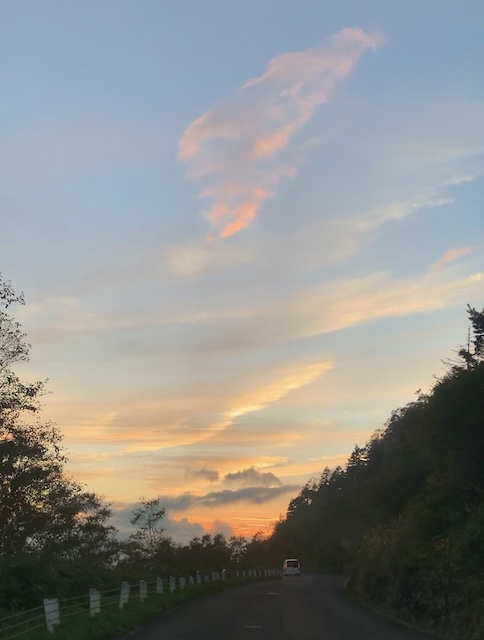
\includegraphics[width=6cm]{sections/Nakahara/IMG_8501.jpg}
\centering
\caption{ドライブ中の車窓から}
\end{figure}

ドライブを楽しんでいたら、クオレの夕食の時間に間に合わないことに気付き、電話をかけようとしましたが、標高が高いせいか電波が届きませんでした。旅にトラブルはつきものだなと思いました。結局夕食の時刻ちょうどくらいに電話をすることになりましたが、クオレさんには優しく許していただけました。その節は大変ご迷惑をおかけしました。

クオレに着くと早速夕食で、焼きそば、焼肉、お米が用意されており、夜の天体観測に備えて満腹になるまでしっかり食べました。とても美味しかったです。
\begin{figure}[H]
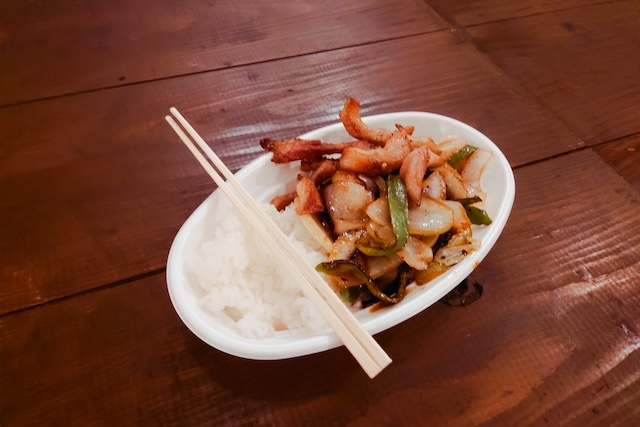
\includegraphics[width=8cm]{sections/Nakahara/IMG_8502.jpg}
\centering
\caption{1日目の夕食}
\end{figure}

クオレさんには諸事情で、電通大天文部であることを伝えていなかったのですが、3度目の訪問であること、一度会えば忘れることは難しい、オレンジ好きが高じてずっとオレンジ色のものを身につけている部員がいたことで、クオレさんには一目でバレてしまいました。「あ、そういうこと?」と全てを察していた場面は面白かったですね。

夕食を終えて風呂に入り、天体観測をはじめました。が、あいにくの天気で満足いくほど星を見ることはできませんでした。それでも夏の天の川は肉眼でも見え、僕の大好きな冬の星空も雲の間からその姿を見せてくれました。たとえ曇っていても、都会から離れ光害の少ないところで見る満点の星はとても綺麗です。あの景色は何度見ても毎度同じように感動できます。星を見に行くことを全ての人におすすめしたいです。

初日は午前3時には眠ったと思います。僕はクオレさんの朝の景色が好きなので5時半には起床し、桟橋で湖に映る磐梯山でも見ようかと思っていました。朝食の準備がされていたので、献立が気になり覗いてみると、コーヒーを入れて下さったので、桟橋の椅子に座りコーヒーを飲みながらのんびり朝を過ごしました。あのコーヒーは格別でした。

\begin{figure}[H]
\centering
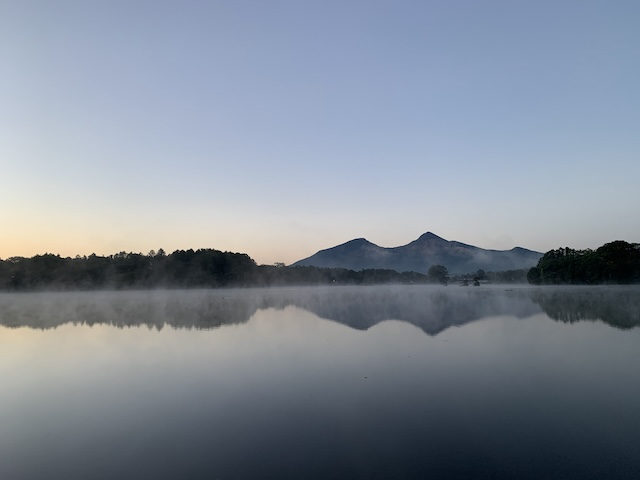
\includegraphics[width=8cm]{sections/Nakahara/IMG_2643.jpeg}
\caption{朝のクオレから見る曽原湖と磐梯山}
\centering
\end{figure}

\subsection{2日目}
2日目は福島観光組と磐梯山登山組に別れました。

1日目の夕食中に、クオレさんに2日目に磐梯山を登る予定であることをクオレさんに話すと、険しくない表磐梯ルートでは幼稚園の遠足で上るレベルなので、登山靴を持っていない人も登れるとアドバイスを頂きました。その結果、当初修士1年3人で登山の予定でしたが、3年生の2人も参加することになりました。修士3人は険しいルート、3年生2人は表磐梯ルートで登山を楽しみました。
登山中は湖や、火山っぽい岩肌、段々と背が低くなる草木を見て楽しみました。途中温泉の匂いがしました。
頂上付近で3年生組とも合流し下山は同じルートでした。3年生のE君は初めての登山でかなりしんどかったらしく、「2度と登山はしない」と誓っていました。

頂上ではしばらく景色を楽しんだり、カップラーメンを食べたり、写真を撮ったりしました。
下に見える雲の間から山や湖が見えるのが綺麗でした。これまでの合宿では、磐梯山はただ眺めるだけのものだったので、登ることができてよかったです。
\begin{figure}[H]
\centering
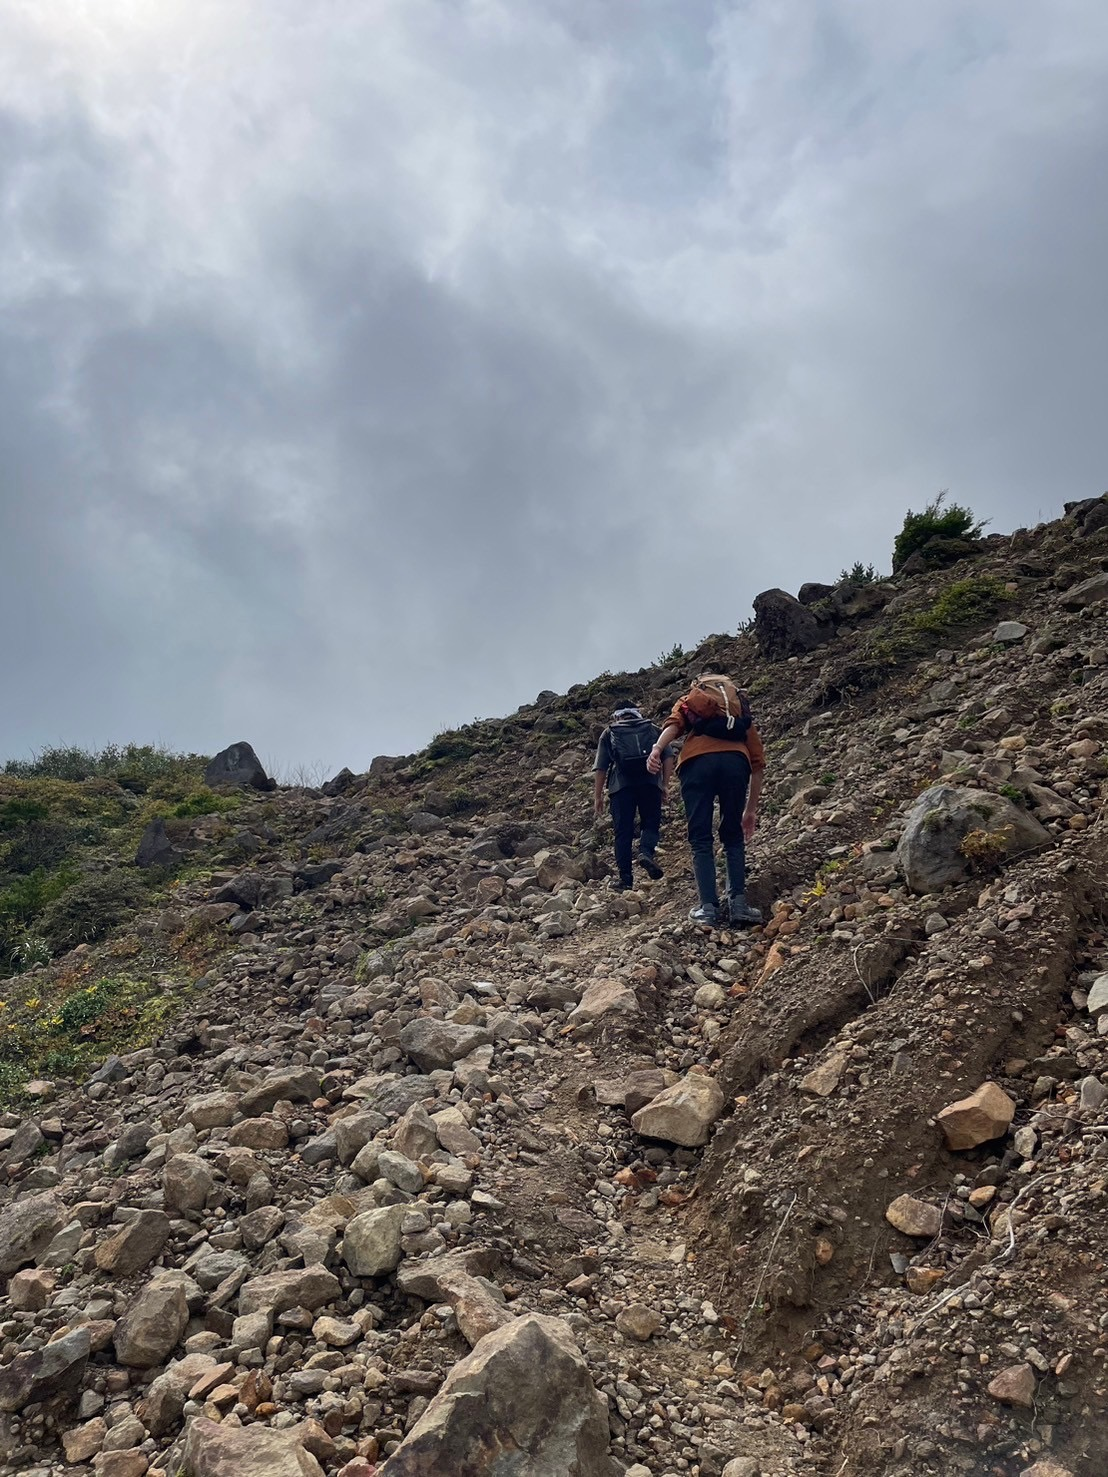
\includegraphics[width=6cm]{sections/Nakahara/IMG_8389.jpg}
\caption{登山の様子}
\centering
\end{figure}

福島観光組は、喜多方ラーメンと温泉を楽しんでいたようです。あまり詳しく聞いていませんが、みんな仲良く楽しそうだったので、良い思い出になったのではないでしょうか。

全員が宿に戻ってきて、夕食をいただき、1日目と同じように天体観測を始めました。が、またまた天気に恵まれませんでした。こればっかりは運なので仕方ないですね。曇っていると気温がそこまで下がらないので、星空を眺めながら椅子にもたれて寝ました。しばらく晴れを待ちましたが、雲はどんどんと厚みを増すばかりだったので、午前3時には寝ました。

\subsection{3日目}
2日目と同じくらいに起き、またコーヒーを頂きました。この時間が一生続けばいいのになと思うくらい良い時間でした。

朝食も美味しくいただき、集合写真を撮ってもらい、ホテルを後にしました。電通大天文部であることを知らせず、得体のしれない集団だったにもかかわらずとても親切にしてくださったクオレさんには感謝してもしきれません。

帰り道の途中で、茨城のビーチに寄り少しだけ景色を楽しんだあと海鮮丼を食べました。少々値段は張りましたが美味しかったですね。僕はブリとマグロの煮切り漬け丼とマグロのユッケを食べました。
\begin{figure}[H]
\centering
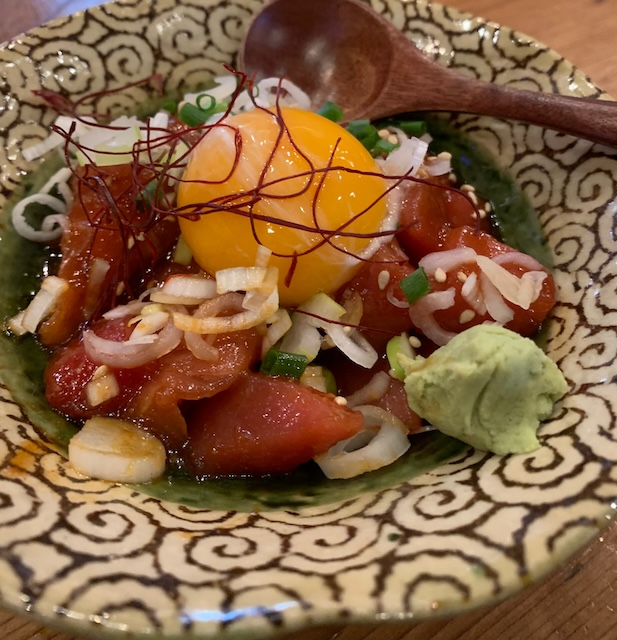
\includegraphics[width=6cm]{sections/Nakahara/yukke.jpeg}
\caption{マグロユッケ}
\centering
\end{figure}
3日目の帰路は大きな渋滞にはまることもなく、無事調布まで戻ってくることができました。事故や怪我がないのが一番ですね。

\section{まとめ}
初めてのレンタカーでの合宿でした。行動の自由度が上がるのは良いですが、翌日の運転のことを考えると天体観測で徹夜ができないのは良くないですね。今回は天気に恵まれなかったので、大人しく寝ることができましたが、快晴だったらおそらく全員がずっと起きていて、運転が不安だったと思います。一長一短ですねぇ。\footnote{個人的には、二泊三日の間寝ずに楽しんで、帰りのバスで思いっきり寝る貸切バスでの合宿が好きです。なんの心配もなく楽しめるのが最高ですね}

9月はあまり天気が良くないことと、夏の天の川が早くに沈んでしまうことを考えると来年は7月か8月に夏合宿をしたいですね。冬の星空も捨てがたいですが...。

夜の天気には恵まれませんでした\footnote{今年の天文部は天候に恵まれず新しい天体写真が少なくて調布祭に展示するものがなくて困ってる人たちがいるらしい}が、磐梯山を登り、絶景を楽しめたので個人的には良い合宿でした。
主催の恵木君や、レンタカーの手配や計画をたててくれた人たちに感謝します。またクオレに行きたいです。


\section{番外編〜天体観測への持ち物〜}
午前2時踏切に〜望遠鏡を担いでった〜〜
(天体観測 BUMP OF CHICKEN)


天体観測には望遠鏡を担いでいくというイメージが多いのではないでしょうか、しかしながら、望遠鏡を担いでいくと、それを支える大きくて重い三脚と赤道儀も担いでいかなければいけません。いきなりそんなガチガチの天体観測は嫌だ!(というかそんな道具は持ってない!)という人に向けて天体観測する時の持ち物を紹介しようと思います!

\subsection{必要なもの}
\subsubsection{防寒具}
真夏を除いて、夜は寒いです。寒い夜に星を見ながらじっとしているとそれはそれは想像を絶する寒さです。天体観測初心者の時は、夜の寒さを舐めてかかり、痛い目に会いました。また、寒さに耐えられなくなり、車や建物の中に戻り、一度快適さを味わうともう外には戻って来られません。夜通し天体観測を行った者しか味わえない特別な朝日を見るために、防寒具は欠かせません。

では、具体的にどのくらいの防寒具を用意しているか紹介します。まず衣類ですが、僕は9月末や3月中旬の合宿では上はヒートテックの上に、長袖Tシャツ2枚、パーカー、ダウンジャケット、下はヒートテックにスウェット、ジーンズ、風を通しにくい素材のズボンを重ね着し、靴下は2枚重ねです。また、パーカーのフードをかぶる、マフラーやネックウォーマーで首を温めることも大事です。

次に衣類以外です。体感ですが、カイロはあまり役に立ちません。持っていかなくていいです。寝袋があると、寝転がって天体観測できるのであると良いです。

\subsection{あると良いもの}
必要なものを考えたら防寒具だけでした、身一つあればできる趣味っていいですね!

\subsubsection{折りたたみ椅子}
ブルーシート敷いて寝袋に入るのもいいんですけど、地面に接してると寒いです。立ちっぱなしで過ごすには夜は長いすぎるので寝転がるか座るかしたい時に、折りたたみ椅子はおすすめです。
カメラで撮影する場合も、寝転がっているとカメラや望遠鏡の操作ができませんが、椅子に座っていれば簡単な操作ぐらいならできます。

座ったまま星を見上げたいので、深く座ることができる背もたれ付きの椅子が良いでしょう。通販でも3000から5000円あれば購入できるのでかなりおすすめです。

\subsubsection{食べ物、カフェイン入りの飲み物}
19時に夕飯を済ませたとすると、翌朝の朝ごはんまで10時間以上は空くことになります。お腹が空くことは当然として、体にエネルギーを入れてあげないと、どんどん寒くなります。そこでチョコレートやクッキーなど簡単に食べられるものを用意しておくと良いでしょう。みんなで食べ物をシェアするのも夜のピクニックみたいで楽しいので、ぜひおすすめのお菓子を持ち寄ってください。

徹夜をしようとするとどうしても眠くなるので、コーヒーやエナジードリンクなどでカフェインを摂るのも良いでしょう。個人的にはチョコレートやクッキーと一緒にピクニック気分を楽しみたいので、コーヒーを用意することが多いです。また、朝の景色を眺めながらのコーヒーは格別なので、最高の朝を過ごしてください。

\subsubsection{双眼鏡}

見えないものを見ようとして望遠鏡を覗き込んだ〜 (天体観測 BUMP OF CHICKEN)

ここまで、お菓子だのコーヒーだの全然星を見ることと関係ないものでした。ようやく天体観測っぽい道具の登場です!

双眼鏡で夜空を見ると、星一つ一つを鮮明に、明るく見ることができます。また、プレアデス星団などの明るめの星団や銀河も双眼鏡で観察することができます。肉眼では見えない天体を見たり、小さな天体を大きく見たりするだけでなく、その位置を手軽に確認するのにも役立ちます。

10月の中旬ごろの紫金山・アトラス彗星を見る時にも、部の双眼鏡を使うことでその尾をはっきりと確認することができました。

\subsubsection{天気予報}
ベルトに結んだラジオ〜雨は降らないらしい

Oh yeah ah

Ah ah ah ah yeah yeah


(天体観測 BUMP OF CHICKEN)

天体観測する前に天気はしっかり確認しておきましょう。

ラジオでじゃないですよ、星を見るのに良い「晴れ」は普通の天気予報の「晴れ」ではなく、快晴レベルである必要があります。scwや星空指数(検索すると出てくる)などで、「晴れ」なのかしっかり確認しましょう。


\subsubsection{友達}

今というほうき星

君と2人追いかけている

Oh yeah ah

Ah ah ah ah yeah yeah


(天体観測 BUMP OF CHICKEN)

夜は1人だと心細いし、退屈になってくるので、是非友達と出かけることをお勧めします。






\end{document}
